\documentclass[aspectratio=169, 11pt]{beamer}

% --- Packages & Setup ---
\PassOptionsToPackage{table}{xcolor}
\usepackage[utf8]{inputenc}
\usepackage[T1]{fontenc}
\usepackage{xcolor}
\usepackage{colortbl}
\usepackage{booktabs}
\usepackage{graphicx}
\usepackage{tikz} % Required for the corner box
\usetikzlibrary{calc,arrows.meta,positioning,shapes.geometric,fit,backgrounds,decorations.pathreplacing}
\usepackage{array}
\usepackage{pgfplots}
\pgfplotsset{compat=1.17}

% Try loading Open Sans; fallback if missing
\IfFileExists{opensans.sty}{\usepackage[default,scale=0.95]{opensans}}{}

% --- Branding Colors ---
\definecolor{amritaMaroon}{HTML}{A4123F}

% --- Theme Setup ---
\usetheme{Madrid}
\usecolortheme[named=amritaMaroon]{structure}
\setbeamertemplate{navigation symbols}{}
\setbeamertemplate{footline}[frame number]
\setbeamertemplate{itemize items}[circle]
\setbeamerfont{footnote}{size=\tiny}

\newcommand{\srcnote}[1]{{\footnotesize\color{gray}\textit{#1}}}

\begin{document}

% --- CUSTOM TITLE SLIDE (Research) ---
\begin{frame}
    % Corner Box Indicator
    \begin{tikzpicture}[remember picture,overlay]
        \node[fill=amritaMaroon, text=white, font=\bfseries\footnotesize, anchor=north east, rounded corners=2pt, inner sep=5pt]
        at ($(current page.north east) + (-0.2cm,-0.2cm)$)
        {Type 1: Research Project};
    \end{tikzpicture}

    \centering
    \IfFileExists{logo.png}{\includegraphics[width=3.5cm]{logo.png}}{}
    \vspace{0.3cm}

    {\Large \textbf{\textcolor{amritaMaroon}{A Multi-Protocol Cyber-Deception Framework Combining \\ Language-Model Response Synthesis with \\ Blockchain-Anchored Forensic Logging}}} \\
    \vspace{0.2cm}
    {\normalsize \textbf{Team Number: 58}} \\
    \vspace{0.5cm}

    % Student Table
    \begin{table}
        \centering
        \small
        \renewcommand{\arraystretch}{1.2}
        \begin{tabular}{|c|c|l|}
            \hline
            \textbf{S.No} & \textbf{Register Number} & \textbf{Student Name} \\
            \hline
            1 & CB.SC.U4CSE23129 & Sisir Reddy Nellore \\
            \hline
            2 & CB.SC.U4CSE23611 & Pranav Sharma Chouduru \\
            \hline
            3 & CB.SC.U4CSE23127 & Surya Tejeswar Reddy Nagireddy \\
            \hline
            4 & CB.SC.U4CSE23111 & Guru Sai Prasad Reddy Bompalli \\
            \hline
            5 & CB.SC.U4CSE23644 & Vishnu Sathwick Rajala \\
            \hline
        \end{tabular}
    \end{table}
    \vspace{0.3cm}

    Guide: \textbf{Dr. Radhika G} \\
    {\footnotesize Department of CSE}

    \vspace{0.5cm}
    {\footnotesize \today}
\end{frame}

% ============================================================
\section{Problem Statement}
\begin{frame}{Problem Statement}
    Low- and medium-interaction honeypots answer from a \textbf{fixed, deterministic response table} --- cheap and safe, but structurally enumerable.
    \begin{itemize}
        \item \textbf{Fingerprintable by design.} Vetterl and Clayton fingerprinted low/medium-interaction honeypots at Internet scale with a \emph{single packet}, equal-error rate 0.0183, locating 7{,}605 instances across nine implementations.
        \vspace{2mm}
        \item \textbf{Single-surface LLM deception.} Generative honeypots that exist (ShelLM, HoneyGPT, HoneyLLM) target one Linux shell each --- no shared engine spans multiple heterogeneous protocols.
        \vspace{2mm}
        \item \textbf{Untrustworthy forensic logs.} A honeypot's entire purpose is to be attacked; a compromised host can have its own logs silently edited, destroying the evidentiary value of what it captured.
    \end{itemize}
\end{frame}

% ============================================================
\section{Objective}
\begin{frame}{Objective}
    Build a deployable, multi-protocol deception framework that stays convincing under probing and produces a tamper-evident audit trail:
    \begin{itemize}
        \item \textbf{Cover five distinct attack surfaces} --- SSH, an internal AI API, PostgreSQL, an Ethereum JSON-RPC node, and Jenkins CI/CD --- behind one logging proxy.
        \item \textbf{Stay fast where routine, smart where novel.} Answer common traffic at static-honeypot speed; reserve LM generation for genuinely novel input.
        \item \textbf{Anchor forensic integrity independently of the host.} Hash and commit every record on-chain so tampering is detectable even if the honeypot itself is compromised.
        \item \textbf{Classify intent transparently.} Label every interaction with an auditable, rule-based classifier suitable for forensic use.
        \item \textbf{Evaluate honestly.} Measure latency, diversity, realism, and cost as separate axes on real payloads --- and report the failures, not only the favourable numbers.
    \end{itemize}
\end{frame}

% ============================================================
\section{Related Work}
\begin{frame}{Research Gaps We Address}
    \begin{itemize}
        \item \textbf{Generative deception is single-protocol.} ShelLM, HoneyGPT, HoneyLLM and the wider 2023--2025 line apply LM response generation only to an SSH/terminal shell; no prior system applies one engine across five heterogeneous protocols.
        \vspace{2mm}
        \item \textbf{No system couples generation with tamper-evident logging.} Blockchain hash-anchoring is established in digital-forensics logging, but no honeypot-specific paper combines it with a generative decoy layer.
        \vspace{2mm}
        \item \textbf{Realism is reported, rarely interrogated.} Prior work reports a single realism figure without separating what layer of fingerprinting it actually defends against, or admitting the timing signature a tiered design creates.
    \end{itemize}
\end{frame}

\begin{frame}{Comparison Against Cited Systems}
    \scriptsize
    \renewcommand{\arraystretch}{1.3}
    \resizebox{\linewidth}{!}{%
    \begin{tabular}{|l|c|p{4.3cm}|c|c|}
        \hline
        \textbf{System} & \textbf{Surfaces} & \textbf{Response mechanism} & \textbf{Routine latency} & \textbf{Log integrity} \\
        \hline
        Cowrie / Kippo & 1 (SSH) & Static table & Microseconds & None \\
        \hline
        ShelLM & 1 (shell) & Generative & Seconds & None \\
        \hline
        HoneyLLM & 1 (shell) & Generative + filter & 1.88 s mean & None \\
        \hline
        HoneyGPT & 1 (shell) & Generative + state manager & Seconds & None \\
        \hline
        \rowcolor{amritaMaroon!15} \textbf{This work} & \textbf{5} & \textbf{Tiered: static, cache, generative} & \textbf{0.8 ms} & \textbf{On-chain per record} \\
        \hline
    \end{tabular}}
    \vspace{3mm}
    \normalsize
    No prior system spans more than one protocol or anchors its logs. This work is the only one in the comparison that is both multi-surface and tamper-evident.
    \srcnote{Table IV, paper Section 10.4}
\end{frame}

% ============================================================
\section{Architecture}
\begin{frame}{System Architecture --- Overview}
    \small Only the proxy and dashboard are reachable from outside. Decoys, the response engine, the datastore, and the blockchain node sit behind it on an isolated internal network.
    \vspace{1mm}
    \begin{center}
    \resizebox{\linewidth}{!}{%
    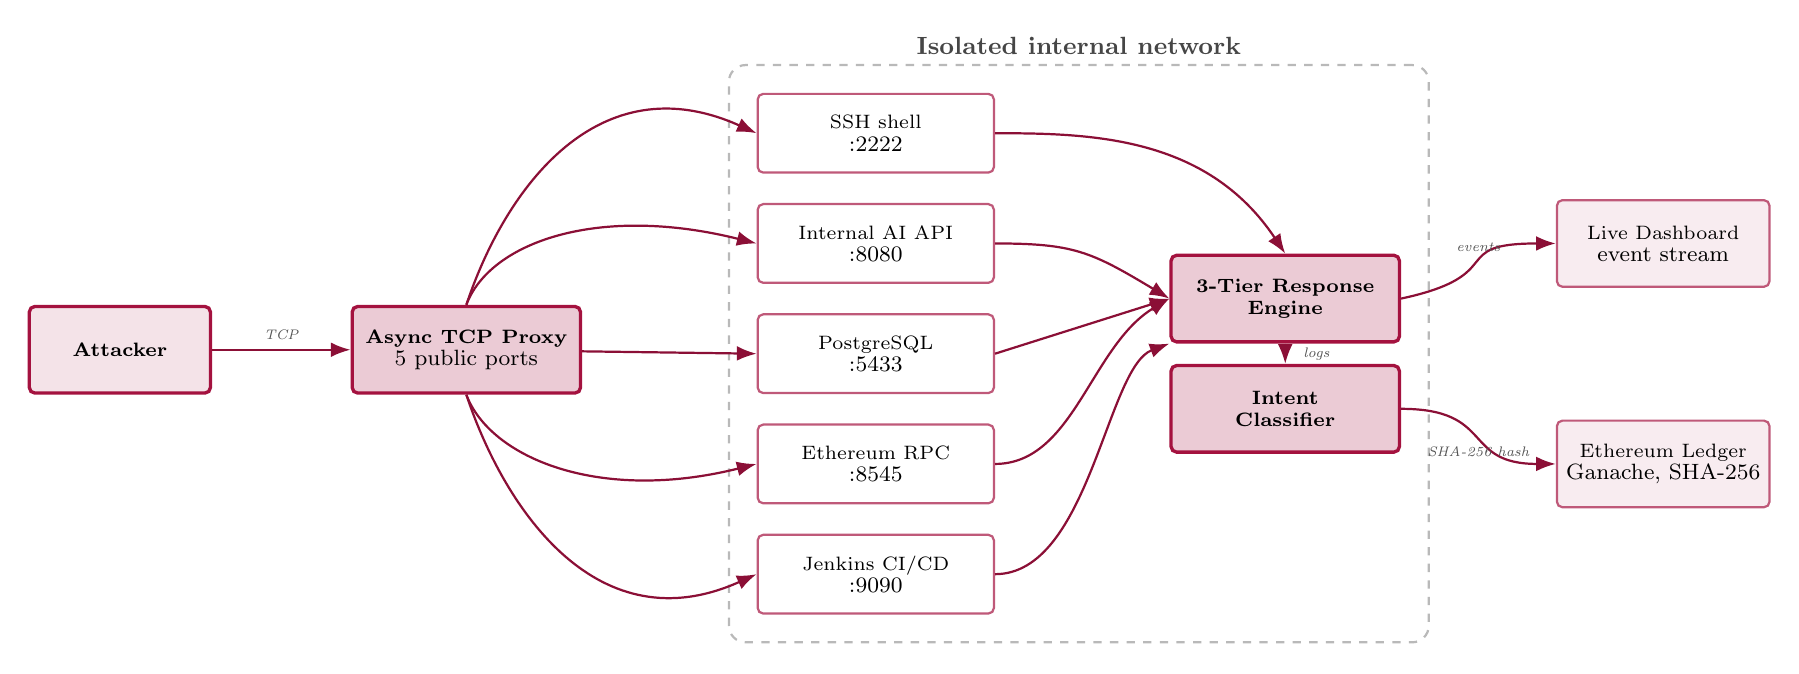
\begin{tikzpicture}[
        font=\scriptsize,
        every node/.style={align=center},
        ext/.style={draw=amritaMaroon, very thick, rounded corners=2pt, fill=amritaMaroon!12,
                    minimum height=1.1cm, minimum width=2.3cm, font=\scriptsize\bfseries},
        comp/.style={draw=amritaMaroon!70, thick, rounded corners=2pt, fill=white,
                     minimum height=1.0cm, minimum width=3.0cm, font=\scriptsize},
        core/.style={draw=amritaMaroon, very thick, rounded corners=2pt, fill=amritaMaroon!22,
                     minimum height=1.1cm, minimum width=2.9cm, font=\scriptsize\bfseries},
        sink/.style={draw=amritaMaroon!70, thick, rounded corners=2pt, fill=amritaMaroon!8,
                     minimum height=1.1cm, minimum width=2.7cm, font=\scriptsize},
        zone/.style={draw=gray!55, dashed, thick, rounded corners=6pt},
        flow/.style={-{Latex[length=2.5mm]}, thick, amritaMaroon!85!black},
        lbl/.style={font=\tiny\itshape, text=gray!65!black}
    ]
        % ================= Column x-positions =================
        % col A: 0        attacker
        % col B: 4.2      proxy
        % col C: 9.2      five decoys (stacked)
        % col D: 14.6     engine / classifier
        % col E: 19.4     dashboard / ledger

        % ---- Column A: external world ----
        \node[ext] (attacker) at (0,-2.75) {Attacker};

        % ---- Column B: public-facing choke point ----
        \node[core] (proxy) at (4.4,-2.75) {Async TCP Proxy\\\footnotesize\normalfont 5 public ports};

        % ---- Column C: decoy layer (internal), stacked top to bottom ----
        \node[comp] (ssh) at (9.6,0)    {SSH shell\\\footnotesize\normalfont :2222};
        \node[comp] (api) at (9.6,-1.4) {Internal AI API\\\footnotesize\normalfont :8080};
        \node[comp] (sql) at (9.6,-2.8) {PostgreSQL\\\footnotesize\normalfont :5433};
        \node[comp] (rpc) at (9.6,-4.2) {Ethereum RPC\\\footnotesize\normalfont :8545};
        \node[comp] (ci)  at (9.6,-5.6) {Jenkins CI/CD\\\footnotesize\normalfont :9090};

        % ---- Column D: response + classification core ----
        \node[core] (engine)     at (14.8,-2.1) {3-Tier Response\\Engine};
        \node[core] (classifier) at (14.8,-3.5) {Intent\\Classifier};

        % ---- Column E: sinks ----
        \node[sink] (dashboard) at (19.6,-1.4) {Live Dashboard\\\footnotesize\normalfont event stream};
        \node[sink] (ledger)    at (19.6,-4.2) {Ethereum Ledger\\\footnotesize\normalfont Ganache, SHA-256};

        % ---- Trust-zone boundary around the internal network ----
        \begin{scope}[on background layer]
            \node[zone, fit=(ssh)(ci)(engine)(classifier), inner sep=10pt,
                  label={[font=\small\bfseries, text=gray!55!black]above:Isolated internal network}] (zone1) {};
        \end{scope}

        % ---- Flows: attacker to proxy ----
        \draw[flow] (attacker) -- (proxy) node[midway, above, lbl] {TCP};

        % ---- Flows: proxy fans out to all five decoys ----
        \draw[flow] (proxy.north) .. controls +(0.5,1.5) and +(-2.0,0.9) .. (ssh.west);
        \draw[flow] (proxy.north) .. controls +(0.3,0.8) and +(-2.0,0.5) .. (api.west);
        \draw[flow] (proxy) -- (sql.west);
        \draw[flow] (proxy.south) .. controls +(0.3,-0.8) and +(-2.0,-0.5) .. (rpc.west);
        \draw[flow] (proxy.south) .. controls +(0.5,-1.5) and +(-2.0,-0.9) .. (ci.west);

        % ---- Flows: decoys into the response engine ----
        \draw[flow] (ssh.east) .. controls +(1.2,0) and +(-1.0,1.5) .. (engine.north);
        \draw[flow] (api.east) .. controls +(1.0,0) and +(-1.0,0.6) .. (engine.west);
        \draw[flow] (sql.east) -- (engine.west);
        \draw[flow] (rpc.east) .. controls +(1.0,0) and +(-1.0,-0.6) .. (engine.west);
        \draw[flow] (ci.east)  .. controls +(1.2,0) and +(-0.8,-0.3) .. (engine.south west);

        % ---- Flows: engine to classifier, classifier to sinks ----
        \draw[flow] (engine.south) -- (classifier.north) node[midway, right, lbl, xshift=1mm] {logs};
        \draw[flow] (classifier.east) .. controls +(1.2,0) and +(-1.2,0) .. (ledger.west) node[midway, below, lbl] {SHA-256 hash};
        \draw[flow] (engine.east) .. controls +(1.4,0.3) and +(-1.4,0) .. (dashboard.west) node[midway, above, lbl] {events};
    \end{tikzpicture}}
    \end{center}
    \srcnote{Paper Section 4}
\end{frame}

\begin{frame}{Five Decoy Services}
    \scriptsize
    \renewcommand{\arraystretch}{1.05}
    \setlength{\tabcolsep}{4pt}
    \begin{tabular}{|l|l|p{7.4cm}|}
        \hline
        \textbf{Decoy} & \textbf{Port / Protocol} & \textbf{Role} \\
        \hline
        SSH shell & 2222 / SSH & Real SSH server; accepts any credentials; interactive shell as a corporate Ubuntu database host; commands route through the response engine \\
        \hline
        Internal AI API & 8080 / REST & Chat/predict endpoints for a fictitious internal model; target for prompt injection and jailbreak attempts \\
        \hline
        PostgreSQL endpoint & 5433 / SQL & Accepts SQL queries; returns plausible tabular results or realistic error text, baiting SQL injection \\
        \hline
        Ethereum JSON-RPC & 8545 / RPC & Responds to the RPC methods attackers invoke to enumerate and drain wallets \\
        \hline
        Jenkins CI/CD & 9090 / HTTP & Build- and script-oriented endpoints representing the documented Jenkins attack surface \\
        \hline
    \end{tabular}
    \vspace{1mm}
    \srcnote{Paper Section 4.2}
\end{frame}

\begin{frame}{Three-Tier Response Path}
    \small Generating every response with the LM would be slow, costly, and, by its uniform multi-second latency, itself detectable.
    \begin{center}
    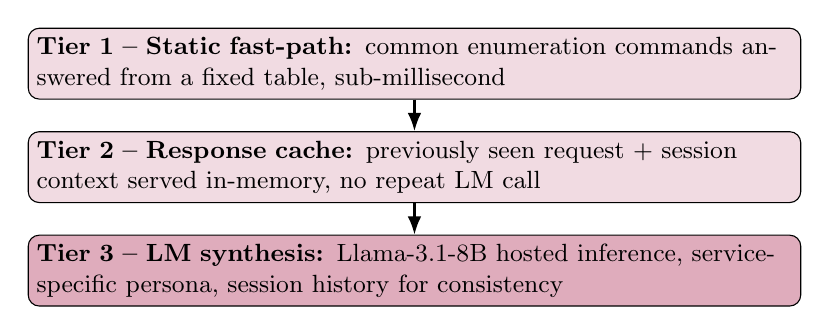
\begin{tikzpicture}[
        node distance=4mm,
        tier/.style={draw, rounded corners, fill=amritaMaroon!15, text width=9.6cm, minimum height=0.9cm, align=left, font=\small, inner sep=3pt},
        arr/.style={-{Latex}, thick}
    ]
        \node[tier] (t1) {\textbf{Tier 1 -- Static fast-path:} common enumeration commands answered from a fixed table, sub-millisecond};
        \node[tier, below=of t1] (t2) {\textbf{Tier 2 -- Response cache:} previously seen request + session context served in-memory, no repeat LM call};
        \node[tier, below=of t2, fill=amritaMaroon!35] (t3) {\textbf{Tier 3 -- LM synthesis:} Llama-3.1-8B hosted inference, service-specific persona, session history for consistency};
        \draw[arr] (t1) -- (t2);
        \draw[arr] (t2) -- (t3);
    \end{tikzpicture}
    \end{center}
    \small\textbf{Intent classification:} rule-based, 8 categories (SQLi, prompt injection, crypto theft, cryptomining, reverse shell/RCE, privilege escalation, supply-chain/CI-CD abuse, reconnaissance) --- auditable and explainable, chosen over a learned classifier for forensic use.
    \srcnote{Paper Section 4.3--4.4}
\end{frame}

\begin{frame}{Blockchain-Anchored Logging}
    \begin{itemize}
        \item Every record is intent-classified, serialised deterministically, and \textbf{SHA-256 hashed}.
        \item The hash is anchored as a transaction on a local Ethereum chain (Ganache); the full record stays in the datastore, only the digest goes on-chain.
        \item Any post-hoc edit to a stored record changes its hash, which no longer matches the on-chain digest --- \textbf{detectable without trusting the honeypot host}.
        \item Integrity, not veracity: the anchor proves a record was not altered after capture. It does not prove the (synthesised) response describes a real system state.
    \end{itemize}
    \vspace{3mm}
    \begin{block}{\small Integrity Test Result}
        \small An untampered record's recomputed SHA-256 digest matched the anchored value exactly. After altering a single field, the recomputed digest diverged from the anchored value --- confirming tamper-evidence.
    \end{block}
    \srcnote{Paper Section 4.5, 6.5, 8.5}
\end{frame}

% ============================================================
\section{Evaluation Methodology}
\begin{frame}{Evaluation Methodology}
    Evaluated the LM-backed dynamic path against a static-response baseline on \textbf{2{,}500 real, publicly documented} attack payloads (SecLists, PayloadsAllTheThings) across all five services.
    \begin{itemize}
        \item \textbf{Four independent axes, kept separate:}
        \begin{itemize}
            \item Latency / sequential throughput and concurrent throughput (10 simultaneous sessions, fresh nonce per request to force a genuine model call)
            \item Response diversity --- uniqueness ratio per service
            \item LM-judge realism --- independent Llama-3.1-70B judge, 1--5 rubric, 30-payload sample
            \item Blockchain integrity --- direct tamper test
        \end{itemize}
        \item Payload split: 1{,}862 SSH, 474 SQL, 136 API, 18 Web3, 10 CI/CD --- capped at the real payloads genuinely available per surface, no padding.
        \item Corpus is \textbf{single-request payloads evaluated independently} --- a stated limitation, not a multi-stage campaign simulation.
    \end{itemize}
    \srcnote{Paper Section 5}
\end{frame}

\begin{frame}{Corpus Coverage by Adversary Behaviour}
    \scriptsize
    \renewcommand{\arraystretch}{1.25}
    \resizebox{\linewidth}{!}{%
    \begin{tabular}{|l|c|p{6.6cm}|c|}
        \hline
        \textbf{Partition} & \textbf{n} & \textbf{Adversary behaviour represented} & \textbf{ATT\&CK} \\
        \hline
        SSH & 1{,}862 & Command injection, shell enumeration, reverse-shell staging, credential access, cryptomining install & T1059.004, T1082, T1071, T1552 \\
        \hline
        SQL & 474 & SQL injection, schema enumeration, authentication bypass, data exfiltration via query & T1190, T1213 \\
        \hline
        API & 136 & Prompt injection, jailbreak, XXE, SSRF against an internal model-serving endpoint & T1190, T1552.001 \\
        \hline
        Web3 & 18 & Wallet enumeration, unauthorised account unlock and transfer against exposed JSON-RPC & T1190, T1657 \\
        \hline
        CI/CD & 10 & Build-system abuse, script-console RCE, credential harvesting from a CI server & T1195, T1059 \\
        \hline
    \end{tabular}}
    \vspace{3mm}
    \normalsize
    Payloads are real strings observed or catalogued in the wild --- the corpus covers the \emph{content} of a broad range of contemporary attacks. It does \textbf{not} cover multi-stage campaigns: every payload is evaluated as a single, independent request.
    \srcnote{Table I, paper Section 5.2}
\end{frame}

% ============================================================
\section{Results}
\begin{frame}{Latency and Throughput}
    \scriptsize
    \renewcommand{\arraystretch}{1.2}
    \begin{tabular}{|l|c|c|}
        \hline
        \textbf{Metric} & \textbf{Static fast-path} & \textbf{Dynamic (LM) path} \\
        \hline
        Mean latency & 0.8 ms & 2.33 s \\
        \hline
        Median latency & 0.8 ms & 1.73 s \\
        \hline
        Std. deviation & 0.3 ms & 1.40 s \\
        \hline
        Sequential throughput & $\approx$1{,}250 req/s & 0.43 req/s \\
        \hline
    \end{tabular}
    \vspace{3mm}
    \normalsize
    The two paths are roughly \textbf{four orders of magnitude} apart --- the explicit justification for tiering: routing routine traffic to the fast-path is what makes an LM-backed honeypot viable at all.
    \vspace{2mm}
    \srcnote{Paper Section 6.1}
\end{frame}

\begin{frame}{Concurrency Scaling: Where the Ceiling Really Is}
    Ten simultaneous sessions sustain \textbf{1.61 req/s} at 2.19 s mean per-request latency (6.21 s wall time for the burst).
    \begin{itemize}
        \item Ideal linear scaling at concurrency 10 would give 4.29 req/s. Measured 1.61 req/s $\Rightarrow$ speedup 3.76$\times$, parallel efficiency 0.376.
        \item Little's Law: requests in flight $= 1.61 \times 2.19 \approx 3.53$, not 10 --- the system saturates at an \textbf{effective parallelism of $\approx$3.5}.
        \item Per-request latency under load (2.19 s) is \emph{lower} than sequential latency (2.33 s) --- if our framework queued requests, load would inflate latency. It does not.
    \end{itemize}
    \begin{block}{\small Diagnosis}
        \small The bottleneck is upstream admission control at the \textbf{hosted inference provider}, not a queue in the proxy, decoys, or response engine. Raising provider concurrency, not re-engineering the framework, is the fix.
    \end{block}
    \srcnote{Paper Section 6.2}
\end{frame}

\begin{frame}{Connection Pooling: Decoy-Layer Latency, All Five Decoys}
    \scriptsize
    \renewcommand{\arraystretch}{1.2}
    \resizebox{\linewidth}{!}{%
    \begin{tabular}{|l|l|c|c|c|}
        \hline
        \textbf{Decoy} & \textbf{Endpoint} & \textbf{Before (mean)} & \textbf{After (mean)} & \textbf{Change} \\
        \hline
        oracle-ai & \texttt{GET /api/models} & 6.15 ms ($\sigma$ 3.89) & 4.28 ms ($\sigma$ 0.70) & $-30.4\%$ \\
        \hline
        vault-sql & \texttt{GET /health} & 0.69 ms ($\sigma$ 1.94) & 0.41 ms ($\sigma$ 0.44) & $-41.4\%$ \\
        \hline
        ledger-trap & \texttt{POST /} (\texttt{eth\_accounts}) & 5.96 ms ($\sigma$ 2.43) & 4.20 ms ($\sigma$ 0.75) & $-29.5\%$ \\
        \hline
        forge-ci & \texttt{GET /api/json} & 6.95 ms ($\sigma$ 3.13) & 6.71 ms ($\sigma$ 3.02) & $-3.4\%$ \\
        \hline
        shadow-shell & SSH \texttt{whoami} & 7.91 ms ($\sigma$ 9.94) & 4.64 ms ($\sigma$ 6.55) & $-41.3\%$ \\
        \hline
    \end{tabular}}
    \vspace{3mm}
    \normalsize
    A single pooled HTTP client, reused for the process lifetime, cut latency by \textbf{30--41\%} on four of five decoys and tightened variance by half to two-thirds. \texttt{forge-ci} barely moves --- it routes through the response engine regardless of decoy-layer pooling, so its floor is the cache lookup.
    \srcnote{Table V, paper Section 11.1}
\end{frame}

\begin{frame}{Response Diversity by Decoy Service}
    \begin{center}
    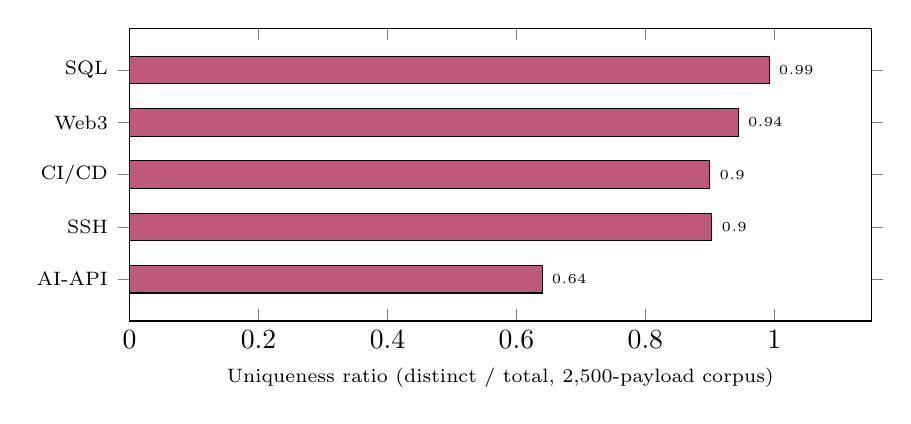
\begin{tikzpicture}
        \begin{axis}[
            xbar, bar width=10pt, width=11cm, height=5.3cm,
            xmin=0, xmax=1.15,
            symbolic y coords={AI-API,SSH,CI/CD,Web3,SQL},
            ytick=data, y tick label style={font=\scriptsize},
            xlabel={Uniqueness ratio (distinct / total, 2{,}500-payload corpus)}, xlabel style={font=\scriptsize},
            nodes near coords, nodes near coords style={font=\tiny},
            enlarge y limits=0.2,
            ]
            \addplot[fill=amritaMaroon!70] coordinates {(0.640,AI-API) (0.903,SSH) (0.900,CI/CD) (0.944,Web3) (0.992,SQL)};
        \end{axis}
    \end{tikzpicture}
    \end{center}
    \textbf{AI-API} is the clear outlier --- a meaningful minority of responses to structurally similar payloads (XXE, SSRF probes) converge on near-identical generic error text.
    \srcnote{Table II, paper Section 6.3}
\end{frame}

\begin{frame}{Per-Service Results: Diversity and Realism Agree}
    \scriptsize
    \renewcommand{\arraystretch}{1.2}
    \resizebox{\linewidth}{!}{%
    \begin{tabular}{|l|c|c|c|l|}
        \hline
        \textbf{Service} & \textbf{Payloads} & \textbf{Distinct outputs} & \textbf{Uniqueness ratio} & \textbf{Judged realism} \\
        \hline
        SQL & 474 & 470 & 0.992 & High \\
        \hline
        Web3 & 18 & 17 & 0.944 & High \\
        \hline
        SSH & 1{,}862 & 1{,}681 & 0.903 & High, small templated minority \\
        \hline
        CI/CD & 10 & 9 & 0.900 & High \\
        \hline
        \rowcolor{amritaMaroon!15} \textbf{AI-API} & \textbf{136} & \textbf{87} & \textbf{0.640} & \textbf{Lowest -- most low ratings} \\
        \hline
    \end{tabular}}
    \vspace{3mm}
    \normalsize
    Mean LM-judge realism: \textbf{4.37/5} ($\sigma=1.45$, $n=30$). Distribution strongly bimodal: 25 rated 5, one rated 2, four rated 1, none rated 3 or 4 --- usually in character, occasionally a complete lapse.
    \srcnote{Table II, paper Section 6.4}
\end{frame}

\begin{frame}{Realism Score Distribution ($n=30$)}
    \begin{center}
    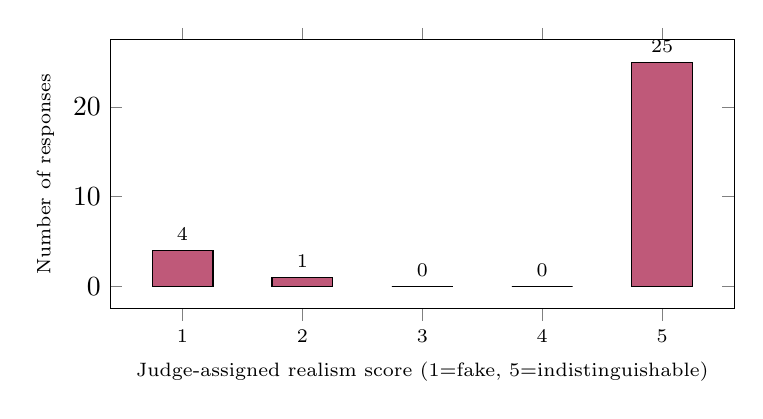
\begin{tikzpicture}
        \begin{axis}[
            ybar, bar width=22pt, width=9.5cm, height=5cm,
            symbolic x coords={1,2,3,4,5},
            xtick=data, xlabel={Judge-assigned realism score (1=fake, 5=indistinguishable)},
            xlabel style={font=\scriptsize}, x tick label style={font=\scriptsize},
            ylabel={Number of responses}, ylabel style={font=\scriptsize},
            nodes near coords, nodes near coords style={font=\scriptsize},
            enlarge x limits=0.15,
            ]
            \addplot[fill=amritaMaroon!70] coordinates {(1,4) (2,1) (3,0) (4,0) (5,25)};
        \end{axis}
    \end{tikzpicture}
    \end{center}
    Low ratings concentrate on, but are not exclusive to, the AI-API decoy: generic error text that ignores the specific XML/SSRF probe, plus a few templated SSH fallbacks.
    \srcnote{Paper Section 6.4}
\end{frame}

\begin{frame}{Blockchain Integrity: Direct Tamper Test}
    Independently of realism and diversity, we verify the tamper-evidence claim directly rather than assuming it holds.
    \begin{itemize}
        \item Fetch a stored record, recompute its SHA-256 digest, and confirm it matches the value already anchored on-chain.
        \item Modify one field of that record, re-hash, and confirm the digest now \textbf{diverges} from the anchored value.
        \item Repeat for a record that was never tampered with, to rule out a false-positive detector.
    \end{itemize}
    \vspace{2mm}
    \begin{block}{\small Result}
        \small For an untampered record the recomputed digest matches exactly. After a single-field edit, the recomputed digest diverges from the anchored value every time --- tampering is detected without trusting the honeypot host that produced the record.
    \end{block}
    \vspace{2mm}
    \small An attacker who compromises the honeypot and edits a stored record \textbf{cannot} make the edited record's hash match what was already committed on-chain. This is integrity, not veracity: the anchor says the record is unaltered, not that its (synthesised) content is true.
    \srcnote{Paper Section 6.5}
\end{frame}

% ============================================================
\section{Fingerprinting Resistance}
\begin{frame}{Resistance to Fingerprinting: Four Layers, One Metric}
    Response diversity is the metric most generative-honeypot papers report. It addresses \textbf{one of four} fingerprinting layers.
    \scriptsize
    \renewcommand{\arraystretch}{1.3}
    \begin{tabular}{|l|p{3.5cm}|p{3.3cm}|c|}
        \hline
        \textbf{Layer} & \textbf{Attack} & \textbf{Our defence} & \textbf{Evaluated?} \\
        \hline
        1. Transport & Protocol-library deviation (Vetterl \& Clayton) & None specific & No \\
        \hline
        2. Timing & Tier-boundary latency ratio & None currently & Quantified; not mitigated \\
        \hline
        \rowcolor{amritaMaroon!15} 3. Content & Response-set enumeration & Generative synthesis, 0.64--0.99 uniqueness & \textbf{Yes} \\
        \hline
        4. Semantic & Cross-command consistency & Session-history prompting & No \\
        \hline
    \end{tabular}
    \vspace{2mm}
    \normalsize
    High response diversity buys resistance to \textbf{one specific, common} class of automated fingerprinting. Two other layers remain open.
    \srcnote{Table III, paper Section 7}
\end{frame}

\begin{frame}{Finding: The Tiered Design Is Its Own Timing Tell}
    The static fast-path answers in \textbf{0.8 ms} ($\sigma=0.3$ ms). The model path answers in \textbf{2.33 s} ($\sigma=1.40$ s). The distributions do not overlap --- separated by $\approx$3.5 orders of magnitude.
    \begin{block}{\small Finding 1 --- a characterised timing side-channel}
        \small Sending two commands, one common (\texttt{whoami}) and one arbitrary, and comparing response times yields a ratio near \textbf{3{,}000} on our system. No real service exhibits that ratio between two commands of comparable output size. \textbf{A single pair of probes is sufficient to detect the tiered architecture with high confidence.}
    \end{block}
    \vspace{2mm}
    This is a direct consequence of the design choice that makes the system economically viable. The tiering that keeps routine traffic cheap is also the clearest fingerprinting surface it presents.
    \srcnote{Paper Section 7.2}
\end{frame}

% ============================================================
\section{Security Analysis}
\begin{frame}{Security Risks the Generative Layer Introduces}
    \begin{itemize}
        \item \textbf{Prompt injection against the decoy.} Attacker input reaches the model's context directly; a successful override converts suspicion into confirmation. The AI-API decoy is the acute case --- it \emph{advertises} itself as model-serving.
        \item \textbf{Cost exhaustion via forced cache misses.} A unique nonce per request defeats the cache and forces a model call every time --- our own benchmark harness does exactly this. At saturated capacity ($\approx$1.6 req/s) an adversary sustains $\approx$\textbf{138{,}000 model calls/day}: a denial-of-wallet attack.
        \item \textbf{Injection into the operator console.} The dashboard renders attacker-influenced, model-generated text; unescaped output is stored XSS against the defender's own console.
        \item \textbf{Integrity is not veracity.} The blockchain anchor proves a record was not altered --- it says nothing about whether the (synthesised) content is true.
    \end{itemize}
    \srcnote{Paper Section 8}
\end{frame}

% ============================================================
\section{Cost Analysis}
\begin{frame}{Cost Analysis}
    \[
    \text{Cost per 1{,}000 interactions} = 1{,}000 \times (1-h) \times c
    \]
    where $h$ = fraction absorbed by the static path + cache, $c$ = price per model call.
    \begin{itemize}
        \item Mean dynamic response $\approx$19 output tokens; per-call cost is a small fraction of a US cent at commodity hosted pricing.
        \item \textbf{We withdraw the original manuscript's unmeasured 80\% fast-path hit-rate estimate.} Our evaluation forced model calls on 2{,}500 distinct payloads by design --- it bounds usage from above, it does not measure a representative $h$.
        \item The benign case is \emph{not} the binding constraint: Section 8 shows an adversary can force $h \to 0$, generating $\approx$138{,}000 calls/day at saturated throughput.
    \end{itemize}
    \begin{block}{\small Necessary architectural feature, not yet built}
        \small A hard cost ceiling with a defined degradation mode (fall back to static responses under attack) is required for any exposed deployment. Its absence is a current limitation.
    \end{block}
    \srcnote{Paper Section 9}
\end{frame}

% ============================================================
\section{Comparison}
\begin{frame}{Comparison With Prior Systems}
    \scriptsize
    \renewcommand{\arraystretch}{1.3}
    \resizebox{\linewidth}{!}{%
    \begin{tabular}{|l|c|c|c|}
        \hline
        \textbf{System} & \textbf{Routine latency} & \textbf{Novel-request latency} & \textbf{Log integrity} \\
        \hline
        Cowrie / Kippo & Microseconds & n/a (static) & None \\
        \hline
        ShelLM (human study) & Seconds & Seconds & None \\
        \hline
        HoneyLLM & 1.88 s mean & 1.88 s mean & None \\
        \hline
        \textbf{This work} & \textbf{0.8 ms} & \textbf{2.33 s mean} & \textbf{On-chain per record} \\
        \hline
    \end{tabular}}
    \vspace{3mm}
    \normalsize
    \textbf{Not a controlled head-to-head} --- each figure reproduced as published, under different hardware/models. What holds: our fast-path matches static-honeypot speed while sitting in the same latency band as published mid-size generative systems on the novel tail, across five surfaces instead of one, with integrity none of them offer.
    \srcnote{Table IV, paper Section 10}
\end{frame}

% ============================================================
\section{Engineering Gaps}
\begin{frame}{Engineering Gaps Found and Fixed}
    \scriptsize
    \renewcommand{\arraystretch}{1.2}
    \resizebox{\linewidth}{!}{%
    \begin{tabular}{|p{3.3cm}|p{7.8cm}|}
        \hline
        \textbf{Gap} & \textbf{Fix and effect} \\
        \hline
        Naive design routed every command to the LM ($\approx$4.0 s mean) & Introduced 3-tier path + pooled HTTP client + shorter generation cap $\to$ $\approx$1.35 s mean \\
        \hline
        Decoy-layer requests opened a fresh connection per call & Connection pooling: $-$30\% to $-$41\% latency on 4/5 decoys, variance cut by half to two-thirds \\
        \hline
        \rowcolor{amritaMaroon!15} Benchmark harness reused payloads $\to$ measured \textbf{cache}, not the model & Fresh nonce per concurrent request $\to$ corrected throughput from ``hundreds of req/s'' to the real 1.61 req/s \\
        \hline
        Intent classifier labelled $\approx$75\% of traffic \texttt{unknown} & Expanded rule categories $\to$ unknown fraction reduced to effectively zero on a 1{,}000-sample \\
        \hline
    \end{tabular}}
    \vspace{2mm}
    \normalsize
    Kept deliberately in the paper: a benchmark silently measuring its own cache is a common, easily missed mistake --- and the same nonce trick is also an attack (Section 8).
    \srcnote{Paper Section 11}
\end{frame}

% ============================================================
\section{Limitations \& Future Work}
\begin{frame}{Limitations \& Validation Roadmap}
    \begin{itemize}
        \item \textbf{Timing side-channel (most serious):} architectural, cheap to exploit, not yet mitigated.
        \item \textbf{AI-API decoy} trails the other four on both diversity and realism --- prompt under-constrained relative to a shell or SQL engine's rigid output format.
        \item \textbf{Transport-layer fidelity unaudited} on 4 of 5 decoys --- the exact layer the strongest published fingerprinting attack operates on.
        \item Realism is measured by an \textbf{automated LM-judge proxy}, $n=30$ --- not a human-subject study.
        \item Corpus is single-request; \textbf{no multi-stage, cross-session consistency} evaluation yet.
        \item Fast-path hit rate $h$ under live traffic is unmeasured; the original 80\% estimate is withdrawn.
    \end{itemize}
    \vspace{2mm}
    \textbf{Next, in order of value:} persona-escape rate (cheapest), human-subject realism study, multi-stage attack chains, timing-jitter mitigation curve, load sweep to $c{=}100$, live-traffic $h$ measurement.
    \srcnote{Paper Sections 12--13}
\end{frame}

% ============================================================
\section{References}
\begin{frame}{References}
    \tiny
    \setbeamertemplate{bibliography item}[text]
    \renewcommand{\baselinestretch}{0.88}\selectfont
    \begin{thebibliography}{99}
        \bibitem{spitzner} L. Spitzner, \textit{Honeypots: Tracking Hackers}, Addison-Wesley, 2002.
        \bibitem{cowrie} M. Oosterhof, ``Cowrie SSH/Telnet Honeypot,'' 2015. \texttt{github.com/cowrie/cowrie}
        \bibitem{dionaea} The Honeynet Project, ``Dionaea: A Malware-Capturing Honeypot,'' 2016.
        \bibitem{vetterl} A. Vetterl and R. Clayton, ``Bitter Harvest: Systematically Fingerprinting Low- and Medium-interaction Honeypots at Internet Scale,'' \textit{Proc. 12th USENIX WOOT}, 2018.
        \bibitem{mckee} F. McKee and D. Noever, ``Chatbots in a Honeypot World,'' arXiv:2301.03771, 2023.
        \bibitem{shellm} M. Sladi\'{c}, V. Valeros, C. Catania, and S. Garcia, ``LLM in the Shell: Generative Honeypots,'' \textit{Proc. IEEE EuroS\&PW}, 2024.
        \bibitem{honeygpt} Z. Wang et al., ``HoneyGPT: Breaking the Trilemma in Terminal Honeypots with Large Language Model,'' arXiv:2406.01882, 2024.
        \bibitem{honeyllm} W. Fan, Z. Yang, Y. Liu, L. Qin, and J. Liu, ``HoneyLLM: A Large Language Model-Powered Medium-Interaction Honeypot,'' \textit{Proc. ICICS}, 2024.
        \bibitem{sok} R. A. Bridges et al., ``SoK: Honeypots \& LLMs, More Than the Sum of Their Parts?,'' arXiv:2510.25939, 2025.
        \bibitem{logprecis} M. Boffa et al., ``LogPr\'{e}cis: Unleashing Language Models for Automated Malicious Log Analysis,'' \textit{Computers \& Security}, vol. 141, 2024.
        \bibitem{nakamoto} S. Nakamoto, ``Bitcoin: A Peer-to-Peer Electronic Cash System,'' 2008.
        \bibitem{sutton} A. Sutton and R. Samavi, ``Blockchain Enabled Privacy Audit Logs,'' \textit{Proc. ISWC}, 2017.
        \bibitem{judge} L. Zheng et al., ``Judging LLM-as-a-Judge with MT-Bench and Chatbot Arena,'' \textit{NeurIPS}, 2023.
        \bibitem{attack} MITRE, ``MITRE ATT\&CK: Adversarial Tactics, Techniques, and Common Knowledge,'' 2015.
        \bibitem{seclists} D. Miessler and J. Haddix, ``SecLists: A Collection of Security Testing Lists,'' 2012.
    \end{thebibliography}
\end{frame}

% --- THANK YOU ---
\begin{frame}
    \centering
    {\Huge \textbf{\textcolor{amritaMaroon}{Thank You}}}
\end{frame}

\end{document}
